\section{Fuels and Energy}

\begin{multicols}{2}


\section*{Transformation of Energy} \index{Energy! transformation of}


\subsection{Chemical to Electrical Energy} \index{Chemical energy} \index{Electrical energy} % LASM

\begin{center}
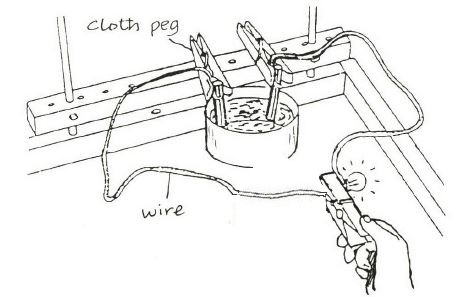
\includegraphics[width=0.49\textwidth]{./img/source/chem-energy.jpg}
\end{center}

\begin{description*}
%\item[Subtopic:]{}
\item[Materials:]{Copper (II) sulphate, zinc metal (from dry cell), copper wire, steel wool, ammeter/bulb}
\item[Setup:]{Prepare a 2 M solution of copper (II) sulphate and clean pieces of copper wire and zinc using steel wool.}
\item[Procedure:]{Connect the zinc anode, ammeter/bulb and copper cathode in series using connecting wires. Dip the zinc and copper electrodes into the copper (II) sulphate solution. Read the current on the ammeter.}
%\item[Hazards:]{}
%\item[Questions:]{}
\item[Observations:]{The ammeter shows a deflection, possibly around 0.05 A.}
\item[Theory:]{The current produced indicates that the chemical energy inherent in the electrodes and the electrolyte solution is converted to electrical energy.}
%\item[Applications:]{}
%\item[Notes:]{}
\end{description*}

\vfill
\columnbreak

\subsection{Making an Electric Heater} \index{Electric heater}

\begin{center}
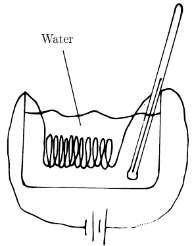
\includegraphics[width=0.3\textwidth]{./img/electric-heater.png}
\end{center}

\begin{description*}
%\item[Subtopic:]{}
\item[Materials:]{Nichrome (resistance) wire (1 m), cardboard tube, speaker wire, 2-4 dry cells, water container, thermometer (optional)}
%\item[Setup:]{}
\item[Procedure:]{Coil the resistance wire around a cardboard tube so that the coils are close but not touching. Use speaker wires to connect the ends of the resistance wire to the terminals of the batteries. Place the coil of resistance wire into the container of water.}
\item[Hazards:]{Do not touch the water when current is flowing. If the heater is connected to the cells while not in the water, the wire can melt or burn other objects.}
%\item[Questions:]{}
\item[Observations:]{By touching the water container \emph{on the outside}, it begins to warm up. If left for long enough, the water will begin to boil.}
\item[Theory:]{The electric heater converts electrical energy into heat energy. The larger the coils are, the more efficient the heater will be.}
\item[Applications:]{Boiling water, heating houses}
%\item[Notes:]{}
\end{description*}

%\subsection{Wind Turbine}
%
%\begin{center}
%\includegraphics[width=0.4\textwidth]{./img/wind-turbine.png}
%\end{center}
%
%\begin{description*}
%%\item[Subtopic:]{}
%\item[Materials:]{30 cm $\times$ 30 cm flexible plastic sheet, pin, scissors, super glue, plastic water bottle, small motor (e.g. from car stereo), connecting wires, galvanometer}
%\item[Propeller:]{Make 5 small holes in the plastic sheet - one at each corner and one in the middle. Cut along the curved lines shown. Fold each corner towards the centre so that all five holes are aligned and glue them in place. Cut the top off of a water bottle just below the lip where the cap sits. Glue the bottle top to the propeller as shown. }
%\item[Generator:]{Make a small hole in the centre of the bottle cap using a pin. Glue the top of the cap to the motor wheel so that the two spin together evenly.}
%\item[Setup:]{Screw the propeller onto the generator like closing a bottle. The propeller should be able to turn freely on the motor. Connect the terminals of the motor to the terminals of the galvanometer.}
%\item[Procedure:]{Hold the propeller upright into the wind so that it spins.}
%%\item[Hazards:]{}
%%\item[Questions:]{}
%\item[Observations:]{The galvanometer will deflect to show that a current is being created in the wire.}
%\item[Theory:]{Mechanical energy (wind) is converted into electrical energy (electric current) using a generator.}
%%\item[Applications:]{Sustainable energy sources}
%%\item[Notes:]{}
%\end{description*}

\vfill
\columnbreak

\subsection{Water Turbine} \index{Water! turbine}

\begin{center}
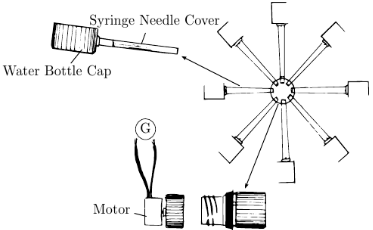
\includegraphics[width=0.45\textwidth]{./img/water-turbine.png}
\end{center}

\begin{description*}
%\item[Subtopic:]{}
\item[Materials:]{Plastic bottle, small motor (e.g. from car stereo), super glue, \nameref{sec:heatsources}, heated nail or soldering iron, 9 water bottle caps, 8 syringe needle caps, scissors, water and pitcher, connecting wires, galvanometer}
\item[Water Wheel:]{Using a hot nail or soldering iron, melt the open end of a syringe needle cap to the side of a water bottle cap to create a sort of spoon. Repeat 7 more times for a total of 8 pieces. Cut the top off a water bottle just below the lip which holds the cap. Melt a plastic cap over the cut end of the bottle top so that the threaded side is open. Use the hot nail or soldering iron to melt 8 holes evenly around the side of this central bottle cap. Insert the 8 spokes into the holes so that they create an 8-spoke wheel with all of the cups facing in one direction at equal distances from the centre. Melt the plastic around each spoke to secure them in place.}
\item[Generator:]{Make a small hole in the centre of the bottle cap using a pin. Glue the top of the cap to the motor wheel so that the two spin together evenly.}
\item[Setup:]{Screw the water wheel onto the generator like closing a bottle. The water wheel should be able to turn freely on the motor. Connect the terminals of the motor to the terminals of the galvanometer.}
\item[Procedure:]{Pour water from a pitcher or spout and place the water wheel under the water so that it turns vertically.}
%\item[Hazards:]{}
%\item[Questions:]{}
\item[Observations:]{The galvanometer will deflect to show that a current is being created in the wire.}
\item[Theory:]{Mechanical energy (falling water and subsequent rotating water wheel) is converted into electrical energy (electric current) using a generator.}
%\item[Applications:]{Sustainable energy sources}
%\item[Notes:]{}
\end{description*}

%==================================================================================================%

%\section*{Energy Changes in Chemical Reactions}
%
%
%\subsection{Endothermic and Exothermic Reactions} % Alt = Chemical Kinetics
%
%\begin{center}
%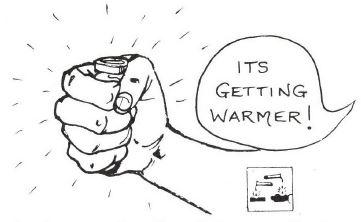
\includegraphics[width=0.4\textwidth]{./img/source/exothermic.jpg}
%\end{center}
%
%\begin{description*}
%%\item[Subtopic:]{}
%\item[Materials:]{3 plastic bottles, powdered soap, citric acid, spoon}
%%\item[Setup:]{}
%\item[Procedure:]{Add a small amount of water to each bottle. Add 3 spoons of powdered laundry soap (e.g. Omo, Foma) to the first bottle. Add 3 spoons of citric acid to the second bottle and nothing to the third bottle. Shake each vigorously and feel to observe any changes in temperature.}
%%\item[Hazards:]{}
%%\item[Questions:]{}
%%\item[Observations:]{}
%\item[Theory:]{The dissolution of laundry soap in water is exothermic -- this bottle should
%get warmer. The dissolution of citric acid is endothermic -- this bottle should get cooler.}
%%\item[Applications:]{}
%%\item[Notes:]{}
%\end{description*}

%\subsection{Endothermic Reactions}
%
%%\begin{center}
%%\includegraphics[width=0.4\textwidth]{./img/.png}
%%\end{center}
%
%\begin{description*}
%%\item[Subtopic:]{}
%\item[Materials:]{Ammonium nitrate, water, container, thermometer (optional)}
%%\item[Setup:]{}
%\item[Procedure:]{Add water to a container or beaker. Add a small amount of ammonium nitrate and stir gently. After all of the ammonium nitrate has dissolved, feel the container or read the thermometer. }
%%\item[Hazards:]{}
%%\item[Questions:]{}
%\item[Observations:]{The container has cooled.}
%\item[Theory:]{This is an example of an \emph{endothermic} reaction. The heat content of the products is greater than the heat contents of the reactants, so the extra energy required is absorbed from the water.}
%%\item[Applications:]{}
%%\item[Notes:]{}
%\end{description*}
%
%\subsection{Exothermic Reactions}
%
%\begin{center}
%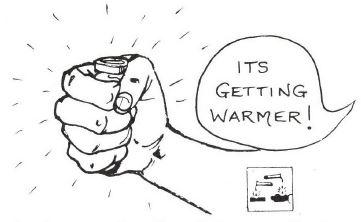
\includegraphics[width=0.4\textwidth]{./img/source/exothermic.jpg}
%\end{center}
%
%\begin{description*}
%%\item[Subtopic:]{}
%\item[Materials:]{Battery acid, sodium hydroxide, bottle, thermometer (optional)}
%%\item[Setup:]{}
%\item[Procedure:]{Add a small amount of water to the container. Carefully pour a small amount of battery acid down the side of the container using a syringe or test tube. Gently stir and \emph{carefully} touch the side of the container or read the thermometer.}
%\item[Hazards:]{The reaction between water and acid produces a lot of heat. Be extremely careful when touching the container. Do not use a highly concentrated acid and always wear goggles.}
%%\item[Questions:]{}
%\item[Observations:]{The container becomes very warm.}
%\item[Theory:]{This is an example of an \emph{exothermic} reaction. The total heat content of the reactants is greater than that of the products, so excess energy is lost to the water.}
%%\item[Applications:]{}
%%\item[Notes:]{}
%\end{description*}

\vfill
\columnbreak

%==================================================================================================%

\section*{Alternative Forms of Energy} \index{Energy! sustainable}


\subsection{Windmills} \index{Windmill}

\begin{center}
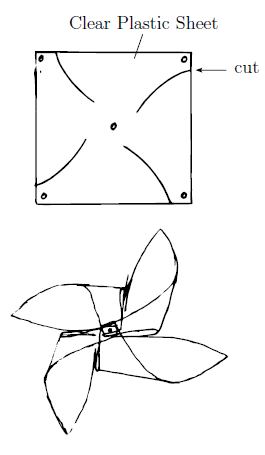
\includegraphics[width=0.35\textwidth]{./img/windmill.png}
\end{center}

\begin{description*}
%\item[Subtopic:]{}
\item[Materials:]{Paper/plastic sheet, scissors, pen, glue, paper fastener/thumb tack, straw or stick}
%\item[Setup:]{}
\item[Procedure:]{Copy the illustration onto a sheet of plastic or paper. Cut along the lines and make holes with a pen. Bend the four corners together into the center and glue them in place. Push the fastener through the center into a straw or stick.}
%\item[Hazards:]{}
%\item[Questions:]{}
%\item[Observations:]{}
%\item[Theory:]{}
%\item[Applications:]{Wind energy, wind turbines (see \nameref{sec:electromagnetism}.}
%\item[Notes:]{}
\end{description*}

%\subsection{Water Wheel}
%
%\begin{center}
%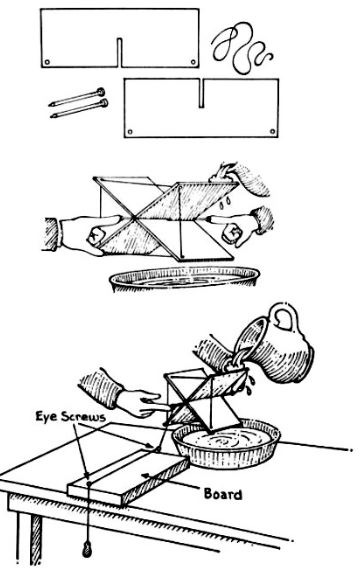
\includegraphics[width=0.5\textwidth]{./img/water-wheel.jpg}
%\end{center}
%
%\begin{description*}
%%\item[Subtopic:]{}
%\item[Materials:]{Stiff cardboard, scissors, nails, string, water, basin}
%\item[Setup:]{Construct the water wheel as shown.}
%\item[Procedure:]{Tie a small weight (e.g. paperclip, nail) to the string so that it rests on the floor. Pour water over the water wheel to turn it and lift the weight. }
%%\item[Hazards:]{}
%%\item[Questions:]{}
%%\item[Observations:]{}
%\item[Theory:]{Water stores potential energy in the forms of rivers and waterfalls and when placed in an elevated storage tank. The kinetic energy of falling water can be used to do work on an object and generate electricity.}
%\item[Applications:]{Water turbines (see \nameref{sec:electromagnetism} (p.~\pageref{sec:electromagnetism}).}
%%\item[Notes:]{}
%\end{description*}


%==================================================================================================%


\end{multicols}

\pagebreak